\documentclass[10pt,a4paper]{extarticle}

\usepackage[margin=1.9cm,top=1.8cm,bottom=1.8cm]{geometry}
\usepackage{booktabs}
\usepackage{longtable}
\usepackage{array}
\usepackage{xcolor}
\usepackage{amsmath}
\usepackage{graphicx}
\usepackage[expansion=false]{microtype}
\usepackage[colorlinks=true,linkcolor=black,urlcolor=blue]{hyperref}
\usepackage{titlesec}
\usepackage{multirow}
% For the same look as the SCAG report, add: \usepackage{lmodern} \usepackage[T1]{fontenc}

\definecolor{srcblue}{RGB}{20,70,140}
\definecolor{good}{RGB}{20,110,70}
\definecolor{warn}{RGB}{170,90,10}
\definecolor{bad}{RGB}{160,40,30}
\definecolor{panel}{RGB}{246,248,250}

\newcommand{\C}[1]{\texttt{\small\detokenize{#1}}}
\newcommand{\src}[1]{\leavevmode{\footnotesize\color{srcblue}\textsf{#1}}}
\newcommand{\ok}[1]{\textcolor{good}{\textbf{#1}}}
\newcommand{\md}[1]{\textcolor{warn}{#1}}
\newcommand{\bd}[1]{\textcolor{bad}{\textbf{#1}}}

\titleformat{\section}{\large\bfseries}{\thesection}{0.6em}{}
\titlespacing{\section}{0pt}{14pt}{5pt}
\titleformat{\subsection}{\normalsize\bfseries}{\thesubsection}{0.5em}{}
\titlespacing{\subsection}{0pt}{10pt}{3pt}

\setlength{\tabcolsep}{5pt}
\setlength{\parindent}{0pt}
\setlength{\parskip}{5pt}
\renewcommand{\arraystretch}{1.15}
\sloppy

\begin{document}

\begin{center}
{\LARGE\bfseries CMAP Planning Network}\\[6pt]
{\footnotesize Chicago Open DTA dataset \quad$\cdot$\quad CMAP trip-based model, c25q4 scenario 100 (2019), PM peak 4--6 pm
\quad$\cdot$\quad October 27, 2026; assignment test added November 6, 2026}
\end{center}
\vspace{4pt}

% =====================================================================
\section{Model fingerprint}

\begin{center}
\begin{tabular}{@{}lr@{\hskip 26pt}lr@{}}
\toprule
\textbf{Source} & & \textbf{Demand} & \\
\midrule
Model                  & CMAP trip-based, ON TO 2050 & Time period             & \textbf{PM} (period 7, 4--6 pm) \\
Scenario               & \textbf{c25q4, 100 = 2019}  & Assignment classes      & \textbf{8} \\
Emme links (directed)  & \textbf{55,005}             & PM vehicle trips        & \textbf{3,527,730} \\
Software               & Emme                        & \quad written ($>$0.01) & 3,481,077 (98.7\%) \\
\addlinespace
\textbf{Driving network} &                           & \textbf{Coding}         & \\
\midrule
Directed GMNS links    & \textbf{55,005} (none dropped) & VDF codes            & 8 \\
Nodes                  & \textbf{20,190}             & Capacity basis          & veh/h/lane, LOS E \\
\quad centroids / road  & 3,649 / 16,541             & VDF                     & CMAP fd1--fd8 \\
Centroid connectors    & 7,264                       & Toll                    & \$ per link, 198 links \\
\addlinespace
\textbf{Zones}         & \textbf{3,649}              & \textbf{Output}         & \\
\midrule
\quad internal / external & 3,632 / 17               & Columns per link        & 30 \\
\quad numbering         & 1--3649, unchanged         & CMAP results kept       & \C{ref_volume}, \C{ref_time} \\
\quad connected         & \ok{all, one strong component} & Gates             & \ok{29 pass, 0 fail} \\
\bottomrule
\end{tabular}
\end{center}

The conversion follows CMAP's own code, not only its documentation. Seven files from CMAP's public model
repository settle what the appendix leaves open: \C{Ftime_capacity.py}, \C{TOD_network_prep.py},
\C{vdf_tod.in}, \C{ttables.mac}, \C{tod_factors.p7}, \C{tod_flags.in} and \C{SOLA_assignment.py}.
Every rule, unit and source is listed in \C{CMAP_network_conversion_reference.pdf}.

% =====================================================================
\section{Reconstruction fidelity}

Each test compares a converted value against a value CMAP itself stored or computed. No assignment is
involved, so this tests the conversion itself.

\begin{center}
\begin{tabular}{@{}lrlc@{}}
\toprule
\textbf{Test} & \textbf{Ours} & \textbf{CMAP's stored value} & \textbf{Agreement} \\
\midrule
\C{DATA1} vs \C{@vadt} & 55,005 links & max difference 0.0005 veh & \ok{exact} \\
\C{TIMAU} vs \C{timau} & 55,005 links & max difference $10^{-6}$ min & \ok{exact} \\
Lanes vs \C{network_p7.txt} & 55,005 / 55,005 & same node and link counts & \ok{exact} \\
\C{@ftime} from binned \C{@speed} & 100\% of VDF 1--6, 8 & \C{Ftime_capacity.py} rule & \ok{exact} \\
VDF 5, 8 at \C{DATA1} vs \C{TIMAU} & median $-0.04\%$ & \C{vdf_tod.in} fd5, fd8 & \ok{exact} \\
PM SOV, mf417 $+$ mf427 $+$ mf437 & 2,351,437 & \C{trip_roster} PM2 mode 1 $=$ 2,351,437 & \ok{exact} \\
OD trips between zones & 3,035,518 & leaving centroids $=$ 3,065,674 & \ok{0.990} \\
\bottomrule
\end{tabular}
\end{center}

The last test closes the loop between demand and network. The 1\% gap is the park-and-ride first legs, which
CMAP builds inside its run and does not export. It also settles one fact the guide leaves implicit:
\textbf{CMAP's stored link volumes are vehicles, not vehicle equivalents}. On a vehicle-equivalent basis the
ratio would be 0.957.

The code also settled four points the appendix states differently or not at all:
\begin{itemize}\setlength{\itemsep}{1pt}
\item \C{@ftime} rounds \C{@speed} up to a speed bin (freeway 70 $\rightarrow$ 65 mph; expressway at least 40);
\item the 0.75 capacity factor applies to VDF 1--5, not only arterials;
\item \C{@toll} is dollars per link;
\item the emmemat period tables mf94--mf97 and mf14--mf18 hold period 8, not PM.
\end{itemize}

% =====================================================================
\section{Network and demand, PM}

\subsection{CMAP's own PM results, by facility}

Read from the converted \C{link.csv} (\C{ref_volume}, \C{ref_time}, \C{vdf_fftt}). Delay is congested minus
free-flow vehicle-hours.

\begin{center}
\begin{tabular}{@{}clrrrrrr@{}}
\toprule
\textbf{VDF} & \textbf{Facility} & \textbf{Links} & \textbf{Lane-mi} & \textbf{VMT} & \textbf{VHT} & \textbf{Delay} & \textbf{Speed} \\
 & & & & {\footnotesize veh-mi} & {\footnotesize veh-h} & {\footnotesize veh-h} & {\footnotesize mph} \\
\midrule
1 & Arterial street         & 41,861 & 36,969 & 16,836,841 & 685,657 & 234,550 & 24.6 \\
2 & Freeway                 & 1,998  & 5,512  & 10,565,352 & 239,959 & 59,891  & 44.0 \\
3 & Freeway $\rightarrow$ arterial ramp & 1,992 & 586 & 364,490 & 15,912 & 3,800 & 22.9 \\
4 & Expressway              & 930    & 1,297  & 1,436,129  & 40,963  & 9,399   & 35.1 \\
5 & Freeway $\rightarrow$ freeway ramp & 664 & 304 & 338,540 & 13,349 & 4,165 & 25.4 \\
6 & Zone centroid connector & 7,264  & 5,052  & 3,893,909  & 194,696 & 0       & 20.0 \\
7 & Toll collection link    & 188    & 82     & 67,954     & 1,254   & 0       & 54.2 \\
8 & Metered entrance ramp   & 108    & 23     & 19,478     & 1,018   & 241     & 19.1 \\
\midrule
 & \textbf{PM, 4--6 pm} & \textbf{55,005} & \textbf{49,824} & \textbf{33,522,694} & \textbf{1,192,807} & \textbf{312,046} & \textbf{28.1} \\
\bottomrule
\end{tabular}
\end{center}

Without connectors, the road network carries 29.6 M VMT at 29.7 mph. In CMAP's PM run, 3,615 road links are
above 1.0 of their VDF capacity, and 2,947 run at more than three times their free-flow time
(Figure~\ref{fig:map}).

\begin{figure}[h]
\centering
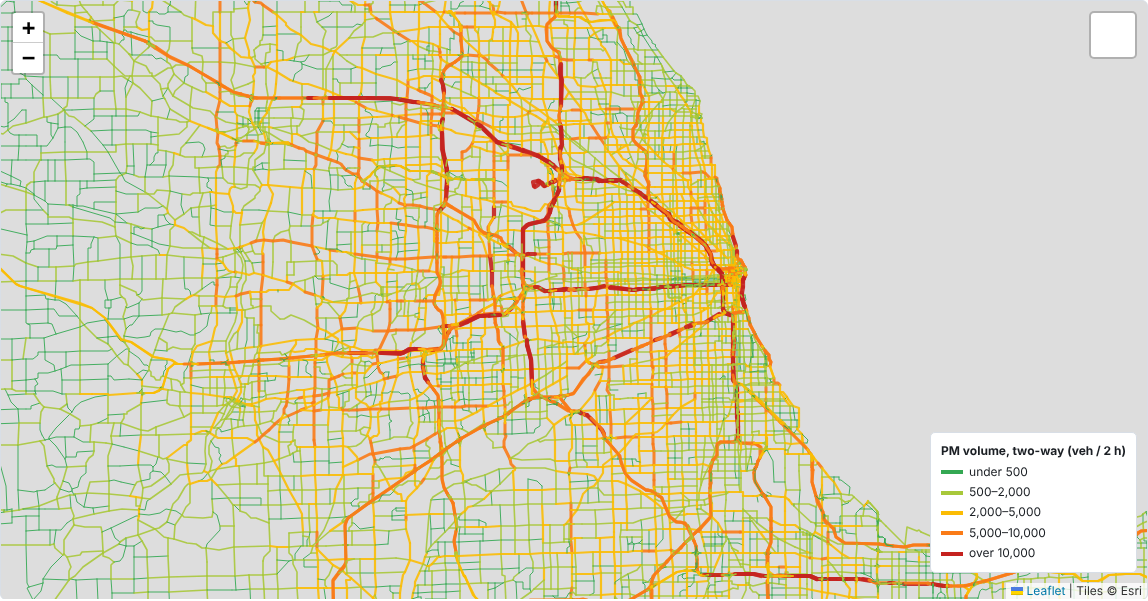
\includegraphics[width=0.495\textwidth]{map_vol.png}\hfill
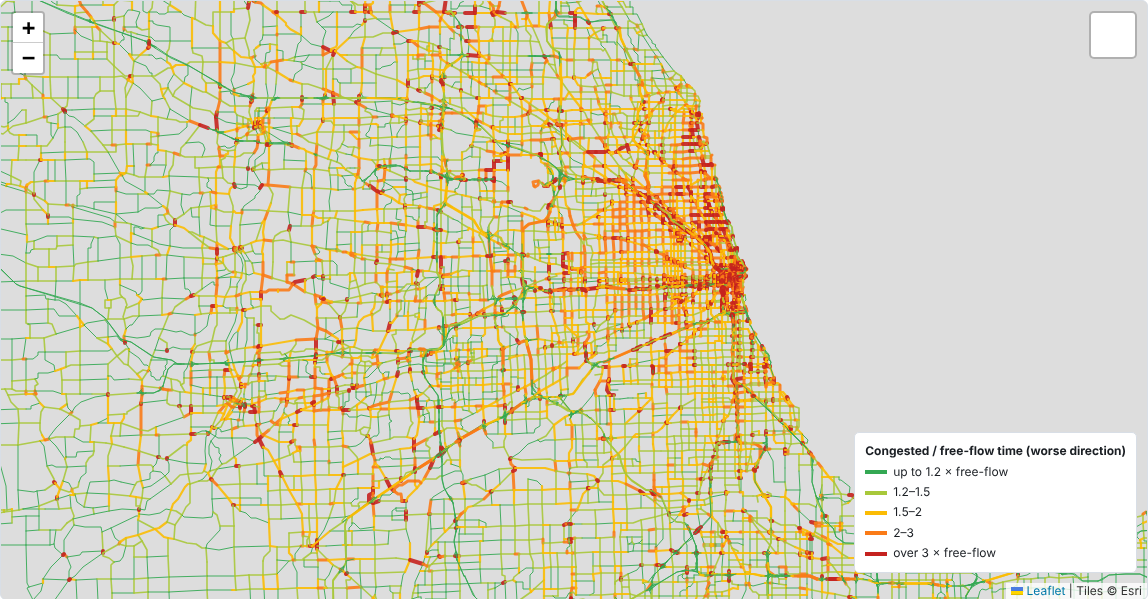
\includegraphics[width=0.495\textwidth]{map_tr.png}
\caption{\footnotesize CMAP's PM assignment, central part of the region, connectors not drawn. Left: two-way
volume. Right: congested over free-flow time, worse direction. Interactive version with the Esri basemap:
\C{CMAP_report.html}.}
\label{fig:map}
\end{figure}

\subsection{Demand}

The PM tables are built the way CMAP's \C{ttables.mac} builds its period-7 tables. The factors come from
\C{tod_factors.p7}, which equal the data guide's TOD7 column. There is one file per class, in vehicles per
2-hour period.

\begin{center}
\begin{tabular}{@{}llrrr@{}}
\toprule
\textbf{Class} & \textbf{Source} & \textbf{PM vehicles} & \textbf{OD rows} & \textbf{Kept} \\
\midrule
\C{sov}  & mf417 $+$ mf427 $+$ mf437 $+\;0.155\times$mf8 (external autos) & 2,393,513 & 818,885 & 100.0\% \\
\C{hov2} & mf447 & 513,112 & 342,932 & 100.0\% \\
\C{hov3} & mf457 & 141,612 & 204,014 & 100.0\% \\
\C{apv}  & $0.155\times$mf10, airport zones only & 11,839 & 26,944 & 99.9\% \\
\C{btrk} & $0.176\times$mf4 (B-plate) & 307,563 & 1,338,781 & 96.5\% \\
\C{ltrk} & $0.176\times$mf5 & 51,627 & 718,863 & \md{71.9\%} \\
\C{mtrk} & $0.176\times$mf6; pce 2 & 48,066 & 664,820 & \md{70.9\%} \\
\C{htrk} & $0.103\times$(mf7 $+$ mf9 external trucks); pce 3 & 60,398 & 659,707 & \md{87.6\%} \\
\midrule
 & \textbf{total} & \textbf{3,527,730} & \textbf{4,774,946} & \textbf{98.7\%} \\
\bottomrule
\end{tabular}
\end{center}

\textbf{Demand floor.} The truck tables are dense: about 13 million positive cells each, most of them a small
fraction of a trip. Cells at or below \textbf{0.01 vehicles} are not written and are not rescaled. Autos keep
over 99.9\%. Light and medium trucks keep about 71\%, and heavy trucks 88\%.

% =====================================================================
\section{Assignment run}

\textbf{First run, preliminary (November 6, 2026).} TAPLite assigned the converted PM network and demand
with one BPR function on every road link. Inputs, the TAPLite build, run scripts and the evaluation are in
\href{https://github.com/hhhhhenanZ/city-tensor/tree/main/cmap_ta_bpr_allmodes}{\C{city-tensor/cmap_ta_bpr_allmodes}}.

\begin{center}
\begin{tabular}{@{}ll@{}}
\toprule
\textbf{Setting} & \textbf{Value} \\
\midrule
Network, demand & this conversion: 55,005 links, 3,649 zones, 3,481,077 PM vehicles (all written cells) \\
Classes & 5: \C{car} $=$ sov $+$ hov2 $+$ hov3 $+$ apv; \C{btrk}, \C{ltrk}; \C{mtrk} (pce 2); \C{htrk} (pce 3) \\
Volume-delay & BPR, $\alpha=0.15$, $\beta=4$, on \C{@emcap} $\times$ lanes; connectors and toll links at \C{@ftime} \\
Tolls, bus preload & not included \\
Run & 10 iterations, relative gap 0.18\,\%, 7 min 43 s on 2 cores, 5.3 GB memory \\
\bottomrule
\end{tabular}
\end{center}

The four car modes are merged into one class because eight classes did not fit in 8 GB (about 8.5 GB
needed). Without tolls the four car modes see the same costs, so link volumes are unchanged; only the split by
car mode is lost.

\begin{center}
\begin{tabular}{@{}lrrrrrr@{}}
\toprule
\textbf{Facility} & \multicolumn{2}{c}{\textbf{VMT (M)}} & \multicolumn{2}{c}{\textbf{VHT (k)}} & \textbf{Speed (mph)} & \textbf{Volume} \\
 & {\footnotesize TAPLite / CMAP} & {\footnotesize ratio} & {\footnotesize TAPLite / CMAP} & {\footnotesize ratio} & {\footnotesize TAPLite / CMAP} & {\footnotesize $R^2$} \\
\midrule
Arterial street   & 15.38 / 16.84 & 0.91 & 427.8 / 685.7 & \md{0.62} & 36.0 / 24.6 & 0.86 \\
Freeway           & 9.96 / 10.57  & 0.94 & 181.0 / 240.0 & \md{0.75} & 55.0 / 44.0 & 0.92 \\
Expressway        & 1.12 / 1.44   & \md{0.78} & 24.8 / 41.0 & \md{0.61} & 45.2 / 35.1 & 0.72 \\
Fwy $\rightarrow$ art.\ ramp & 0.36 / 0.36 & 0.99 & 12.7 / 15.9 & 0.80 & 28.4 / 22.9 & 0.62 \\
Fwy $\rightarrow$ fwy ramp   & 0.30 / 0.34 & 0.88 & 8.7 / 13.3   & 0.65 & 34.3 / 25.4 & 0.74 \\
Toll collection   & 0.07 / 0.07   & 1.04 & 1.3 / 1.3     & 1.05 & 53.8 / 54.2 & 0.90 \\
Metered ramp      & 0.02 / 0.02   & 1.14 & 1.0 / 1.0     & 1.02 & 21.3 / 19.1 & 0.61 \\
\midrule
\textbf{Road links} & \textbf{27.22 / 29.63} & \textbf{0.92} & \textbf{657.4 / 998.1} & \textbf{0.66} & \textbf{41.4 / 29.7} & \textbf{0.93} \\
\bottomrule
\end{tabular}
\end{center}

\begin{figure}[h]
\centering
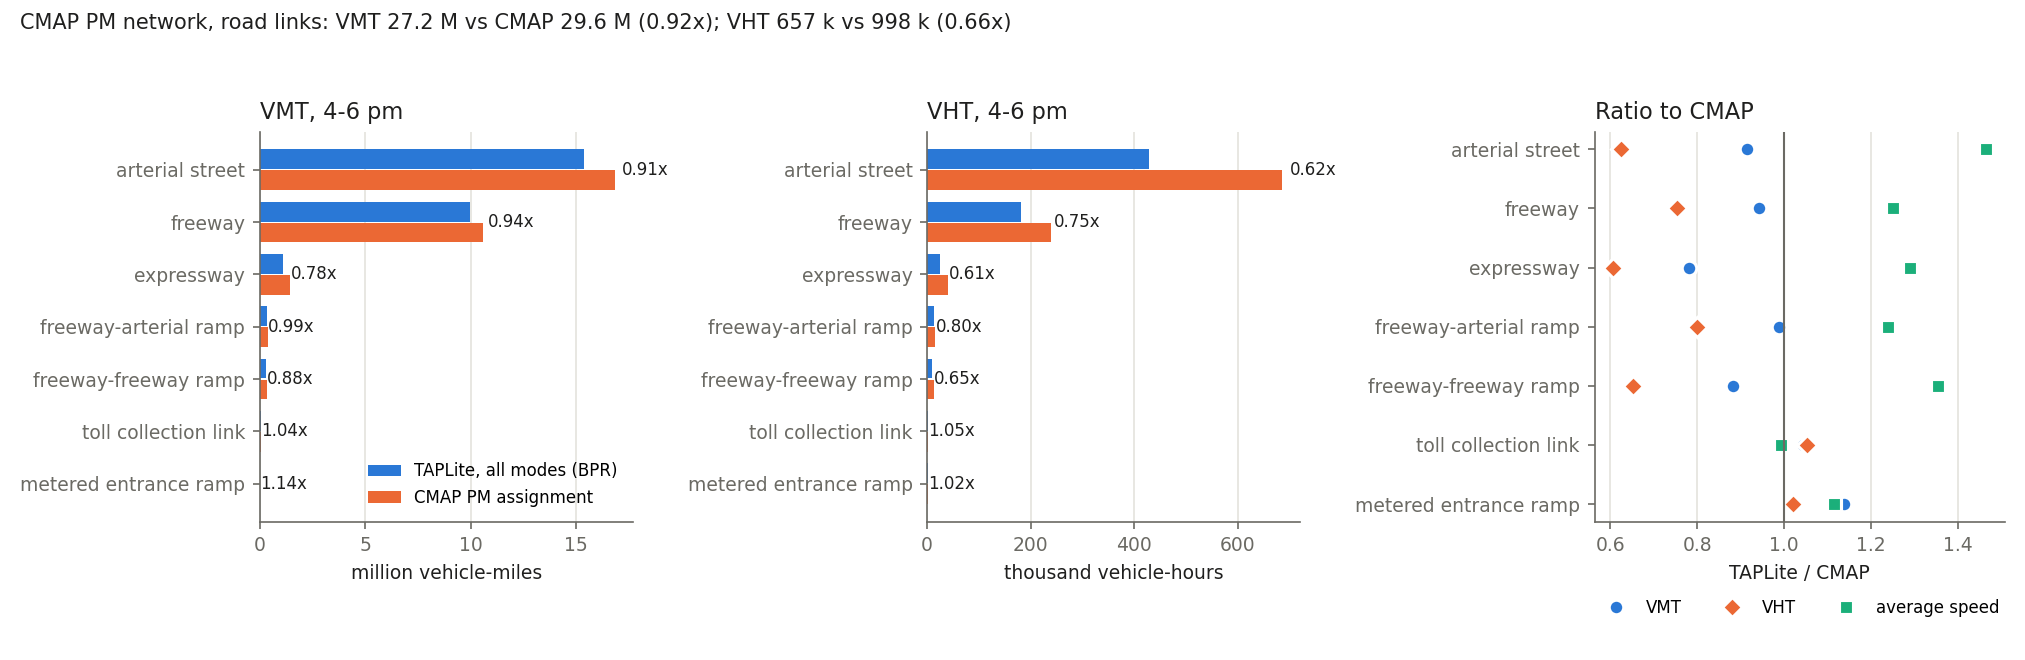
\includegraphics[width=\textwidth]{fig_bpr_vmt_vht.png}
\caption{\footnotesize TAPLite (BPR 0.15, 4) against CMAP's PM assignment by facility type, road links.}
\label{fig:bpr}
\end{figure}

\textbf{Reading.} Route choice is right: volumes follow CMAP on freeways and arterials (VMT 0.94 and 0.91,
$R^2$ 0.92 and 0.86). Delay is not: TAPLite's network delay is 34 thousand vehicle-hours against CMAP's 312
thousand, so speeds are 25--46\,\% higher. Where CMAP has no delay the link times agree; where CMAP is
congested, BPR (0.15, 4) on \C{@emcap} adds much less. CMAP's functions are steeper (0.75 $\times$ capacity,
$\beta=8$ on freeways) and add signal delay on arterials (arterial median time ratio 0.77). Expressways carry
0.78 of CMAP's traffic because the run has no tolls, so the parallel tollways attract more.

\begin{center}
\colorbox{panel}{\parbox{0.96\textwidth}{\vspace{2pt}
Two choices are still open:
\begin{itemize}\setlength{\itemsep}{1pt}
\item \textbf{VDF form.} The BPR test above is too flat. The next candidates are BPR with CMAP's own $\alpha$,
$\beta$ and the 0.75 capacity factor, or a BPR fitted to each CMAP curve (fd1--fd8). CMAP's min-term (fd2, fd4)
and Webster signal delay (fd1, fd3) are not TAPLite functions.
\item \textbf{Bus preload.} CMAP counts buses as 3 vehicle equivalents each (\C{el2}). These are not exported,
so the runs so far are without them.
\end{itemize}\vspace{2pt}}}
\end{center}

% =====================================================================
\section{Model comparison, PM period}

All links including connectors, 4--6 pm. ``Ours'' is the first TAPLite run of Section~4 (BPR 0.15, 4; no
tolls). Delay is congested minus free-flow vehicle-hours.

\begin{center}
\begin{tabular}{@{}lrrrl@{}}
\toprule
\textbf{Measure} & \textbf{Ours} & \textbf{CMAP} & \textbf{Ratio} & \textbf{Reading} \\
\midrule
Demand (vehicle trips between zones) & 3,035,518 & 3,065,674 & \ok{0.990} & park-and-ride legs missing \\
Link volume (vehicles) & 54,301,914 & 56,908,112 & \ok{0.954} & \\
VMT (vehicle-miles)    & 31,016,448 & 33,522,694 & \ok{0.925} & route choice close \\
VHT (vehicle-hours)    & 847,447    & 1,192,807  & \md{0.710} & BPR too flat \\
Delay (vehicle-hours)  & 33,952     & 312,046    & \bd{0.109} & BPR too flat \\
Average speed (mph)    & 36.6       & 28.1       & \md{1.302} & \\
Link volume $R^2$      & \multicolumn{2}{c}{road links} & \ok{0.93} & \\
\bottomrule
\end{tabular}
\end{center}

% =====================================================================
\section{Open items}

\begin{longtable}{@{}p{0.055\textwidth}p{0.45\textwidth}p{0.42\textwidth}@{}}
\toprule
& \textbf{Issue} & \textbf{What would resolve it} \\
\midrule
\endfirsthead
\toprule
& \textbf{Issue} & \textbf{What would resolve it} \\
\midrule
\endhead
\textbf{O1} &
CMAP's arterial function adds Webster delay from the cycle length and $g/C$ at the downstream node
(\C{@cycle}, \C{@gc}, packed into \C{ul3}). Neither is in the export, so arterial times sit 22\% below
\C{TIMAU} at the median. &
The values from CMAP's emmebank, or a rerun of \C{Arterial_delay.py} on the exported network. \\
\addlinespace
\textbf{O2} &
CMAP's link volume includes \C{el2} (buses at 3 veq each), which the PM files do not carry. Freeway and
expressway times reproduce at $-9.5\%$ and $-1.3\%$ without it. &
\C{busveq} from the emmebank, or rebuilt from the transit itineraries. \\
\addlinespace
\textbf{O3} &
Park-and-ride first legs (mf59) are built inside CMAP's run. They are the 1\% gap in the demand loop. &
The convolution in \C{ttables.mac}, run on mf837 and the transit tables. \\
\addlinespace
\textbf{O4} &
The 0.01 floor drops 28--29\% of light and medium trucks. &
A per-origin rescale of the kept cells, or a lower floor (99.7\% kept at 0.0001). \\
\addlinespace
\textbf{O5} &
Scenario 100 is 2019; the speed data is 2023. &
\C{c25q4_200} (2025) has the same file structure, and the same code converts it. \\
\addlinespace
\textbf{O6} &
BPR (0.15, 4) gives 0.11 of CMAP's delay and 0.71 of its VHT. &
CMAP's own $\alpha$, $\beta$ with the 0.75 factor, or a BPR fitted to each of fd1--fd8. \\
\addlinespace
\textbf{O7} &
No tolls in the first run; expressways carry 0.78 of CMAP's VMT. Eight classes need about 8.5 GB. &
Toll as link cost with each class's value of time; run all eight classes on a 16 GB machine. \\
\bottomrule
\end{longtable}

% =====================================================================
\section{Observation alignment and next steps}

Alignment with real-world observations is partly possible already, which is where Chicago differs from SCAG.
The dataset holds 2023 INRIX TMC speeds, hourly, on 18 corridor-directions, with fitted QVDF parameters per
TMC. These are mapped to the OSM City-of-Chicago network today; the next step maps the same TMCs to CMAP
links. \textbf{Counts are still missing}: every corridor demand is derived from speed, and IDOT AADT is the
first independent volume check to add.

\begin{center}
\begin{tabular}{@{}r>{\raggedright\arraybackslash}p{0.22\textwidth}>{\raggedright\arraybackslash}p{0.44\textwidth}l@{}}
\toprule
& \textbf{Stage} & \textbf{What it provides} & \textbf{Status} \\
\midrule
1 & Standardized, documented network & every \C{link.csv} column with source, unit and reference; every CMAP
number in one region file & \ok{complete (PM)} \\
2 & Open executable assignment & TAPLite replay of CMAP's PM assignment & \md{first run (BPR)} \\
3 & Observation alignment & TMC speeds and QVDF on CMAP links; AADT as the volume check & \md{speeds in hand} \\
4 & AI applications & multi-day DTA benchmark (OpenDTA), flow-through tensor, bottleneck detection,
scenario screening & planned \\
\bottomrule
\end{tabular}
\end{center}

\begin{center}
\begin{tabular}{@{}rp{0.80\textwidth}@{}}
\toprule
& \textbf{Next step} \\
\midrule
1 & Rerun the TAPLite PM replay with CMAP-shaped VDFs and tolls (O6, O7); compare volume and time link by link \\
2 & Map the 18 corridor-directions of TMCs onto CMAP links \\
3 & Add IDOT AADT as the first independent volume check \\
4 & Resolve O1--O4 where the emmebank allows \\
5 & Convert AM (period 3) and the 2025 scenario with the same code \\
\bottomrule
\end{tabular}
\end{center}

\vspace{4pt}
{\footnotesize Sources: CMAP Travel Demand Model Data User Guide (c25q4),
\href{https://datahub.cmap.illinois.gov/documents/a14d641dbe184704ab597479b103986c/explore}{CMAP Data Hub};
\href{https://cmap.illinois.gov/wp-content/uploads/ON-TO-2050-Update-Travel-Demand-Model-Documentation-Appendix.pdf}{ON TO 2050 travel demand model appendix};
\href{https://github.com/CMAP-REPOS/cmap_trip-based_model}{CMAP trip-based model code} (commit e52b318).}

\end{document}
